\begin{task}[credit=7]{Regressionsanalyse}
Gegeben sind folgende Datenpunkte:

\begin{table}[h]
\centering
\begin{tabular}{c|cccccccc}
\toprule
\textbf{x} & 1 & 3 & 4 & 6 & 8 & 9 & 11 & 14 \\ \hline
\textbf{y} & 1 & 2 & 4 & 4 & 5 & 7 & 8  & 9  \\
\bottomrule
\end{tabular}
\end{table}

\begin{figure}[h]
\centering
\caption{Veranschaulichung der Datenpunkte zur linearen Regression.}
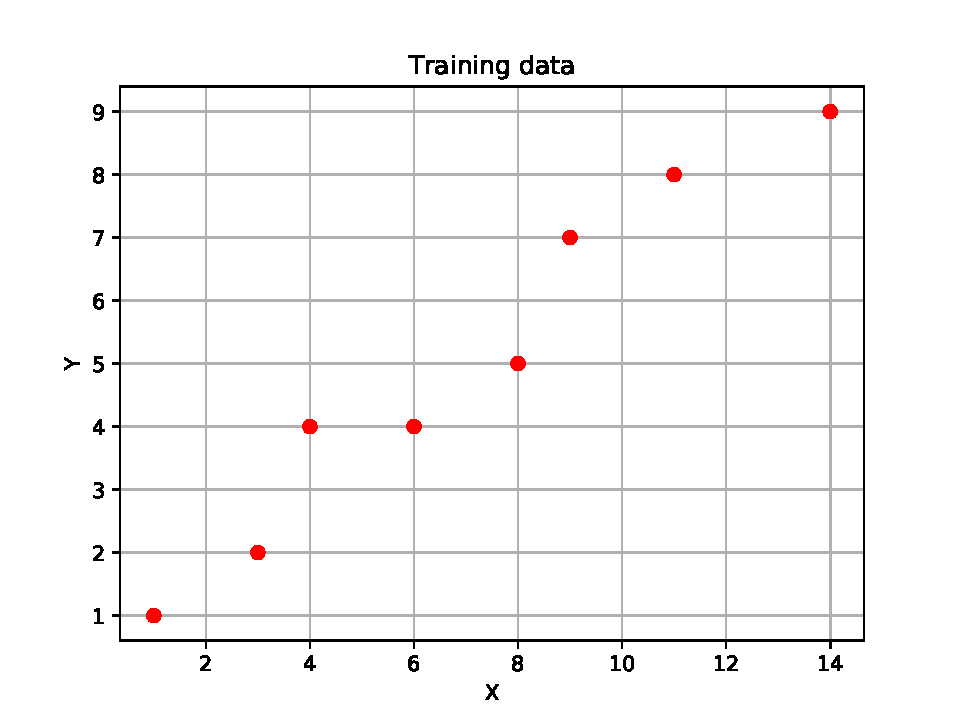
\includegraphics[width=0.5\linewidth]{media/images/data.pdf}
\end{figure}

%We want to build a least square regression model 
Wir möchten eine Regression nach dem Prinzip der kleinsten Fehlerequadrate erstellen:

\begin{equation}
y =f(x)=\left \langle W, x  \right \rangle+b\,.
\end{equation}

Mit der Hilfe eines $(p+1)$-dimensionalen Vektors $\vec{x}=(1, x_1, \cdots , x_p)$ und $x \in \mathbb{R}^{1 \times p}$, können wir $b$ in dem Vektor $W$ codieren:

\begin{equation}
y =f(x)=\left \langle W^{'}, \vec{x}^{T}  \right \rangle,
\end{equation}

wobei hier $W^{'} \in \mathbb{R}^{2 \times 1}$ und $\vec{x} \in \mathbb{R}^{1 \times 2}$.

\begin{subtask}[title=Herleitung,points=5]
 Zeigen Sie, dass das optimale $W^{'}$:
\begin{equation}
W^{'} =  (\vec{X}^{T}\vec{X})^{-1}\vec{X}^{T}Y,
\end{equation}
entspricht, wobei $\vec{X} \in \mathbb{R}^{n \times 2}$ und $Y \in \mathbb{R}^{n \times 1}$.

\begin{solution}
Wir möchten eine Regression nach dem Prinzip der kleinsten Fehlerquadrate erstellen. Das heißt wir wollen folgende Funktion minimieren:
\begin{align*}
\min_{W,b} S(W,b) = \sum_{i=1}^n (W^T x_i + b - y_i)^2.
\end{align*}
Dies ist nach den obigen Definitionen äquivalent zur Minimierung folgender Funktion:
\begin{align*}
\min_{W'} S(W') = \sum_{i=1}^n (W'^T \bar{x}_i - y_i)^2.
\end{align*}
Daraus folgt
\begin{align*}
S(W') &= \sum_{i=1}^n (W'^T \bar{x}_i - y_i)^2 = ||  \vec{X} W' - Y ||^2\\
&= (\vec{X}W' - Y)^T(\vec{X}W' - Y) \\
&= W'^T \vec{X}^T \vec{X}W' - Y^T \vec{X} W' - W'^T \vec{X}^T Y + Y^T Y \\
&= W'^T \vec{X}^T \vec{X} W' - 2 Y^T \vec{X} W' + Y^T Y
\end{align*}
Wir differenzieren nun die Funktion $S(W')$ nach $W'$
\begin{align*}
\frac{\partial S(W')}{\partial W'} &= 2 W'^T \vec{X}^T \vec{X} - 2 Y^T \vec{X}.
\end{align*}
Setzen wir die Ableitung gleich 0 erhalten wir
\begin{align*}
0 &= W'^T \vec{X}^T \vec{X} - Y^T \vec{X} \\
W'^T \vec{X}^T \vec{X} &= Y^T \vec{X} \\
\vec{X}^T \vec{X} W' &= \vec{X}^T Y \\
W' &= (\vec{X}^T \vec{X})^{-1} \vec{X}^T Y
\end{align*}
unter der Bedingung, dass die Inverse $(\vec{X}^T \vec{X})^{-1}$ existiert.
\end{solution}
\end{subtask}


\begin{subtask}[title=Parameterbestimmung,points=2]
Berechnen Sie $W$ und $b$ für den gegebenen Punktdatensatz. Die Inverse $(\vec{X}^{T}\vec{X})^{-1}$ muss dabei nicht manuell berechnet werden.

\begin{solution}
Durch ablesen der Koordinaten erhalten wir: 
\begin{align*}
\vec{X} = 
\begin{pmatrix}
1 & 1 \\
1 & 3 \\
1 & 4 \\
1 & 6 \\
1 & 8 \\
1 & 9 \\
1 & 11 \\
1 & 14 \\
\end{pmatrix}
\text{ und }
\vec{Y} = 
\begin{pmatrix}
1 \\
2 \\
4 \\
4 \\ 
5 \\
7 \\
8 \\ 
9 \\
\end{pmatrix}.
\end{align*}
Daraus folgt
\begin{align*}
\vec{X}^T \vec{X} = 
\begin{pmatrix}
8 & 56 \\
56 & 524 \\
\end{pmatrix}
\text{ und }
(\vec{X}^T \vec{X})^{-1} = 
\begin{pmatrix}
\frac{131}{264} & \frac{-7}{132} \\
\frac{-7}{132} & \frac{1}{132} \\
\end{pmatrix}
\end{align*}
Damit können wir nun W und b berechnen
\begin{align*}
W' &= 
\begin{pmatrix}
\frac{131}{264} & \frac{-7}{132} \\
\frac{-7}{132} & \frac{1}{132} \\
\end{pmatrix}
\begin{pmatrix}
40 \\
364 \\
\end{pmatrix} 
= (\vec{X}^T \vec{X})^{-1} \vec{X}^T Y \\
&= 
\begin{pmatrix}
\frac{6}{11}
\frac{7}{11}
\end{pmatrix}
\end{align*}
Daraus folgt $W= \frac{7}{11}$ und $b = \frac{6}{11}$.
\end{solution}

\end{subtask}
\end{task}
